% tikzpic.tex
\documentclass[crop,tikz]{standalone}% 'crop' is the default for v1.0, before it was 'preview'
%\usetikzlibrary{...}% tikz package already loaded by 'tikz' option
\usepackage{amsmath,amsthm,amssymb,mathrsfs,amsfonts,dsfont}
\usetikzlibrary{plotmarks}

\begin{document}
    % Define macros to store coordinates
    \newcommand{\clusterOnePoints}{}
    \newcommand{\clusterTwoPoints}{}
    \newcommand{\clusterThreePoints}{}

    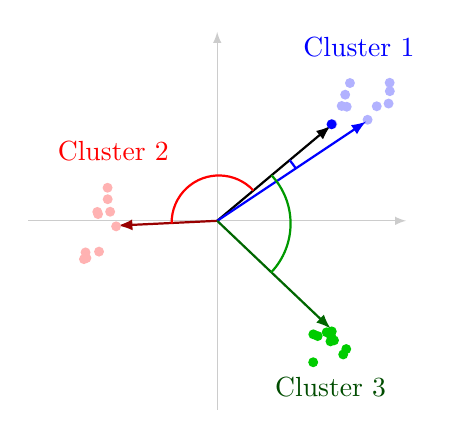
\begin{tikzpicture}[scale=0.6]
        \pgfmathsetseed{170}
        \draw[-latex, gray!40] (-4,0) -- (4,0);
        \draw[-latex, gray!40] (0,-4) -- (0,4);
        % Cluster 1
        \foreach \i in {1,2,...,10} {
            \pgfmathsetmacro{\x}{2 * rnd + 2}
            \pgfmathsetmacro{\y}{rnd + 2}
            \fill[blue!30] (\x,\y) circle (3pt);
            % Append coordinates to \clusterOnePoints
            \xdef\clusterOnePoints{\clusterOnePoints (\x,\y)}
        }
        \node[below, blue] at (3,4.1) {Cluster 1};
        \node[below, red] at (-2.2,1.9) {Cluster 2};
        \node[below, green!30!black] at (2.4,-3.1) {Cluster 3};
        % Show arrows to within and between clusters.
        \draw[-latex, thick, black] (0, 0) -- (2.4, 2.01) ;
        \draw[-latex, thick, blue] (0, 0) -- (3.15, 2.1);
        \draw[-latex, thick, red!60!black] (0, 0) -- (-2.1, -0.1);
        \draw[-latex, thick, green!40!black] (0, 0) -- (2.4, -2.28);
        \fill[blue] (2.42,2.043) circle (3pt);
        
        % Cluster 2
        \foreach \i in {1,2,...,10} {
            \pgfmathsetmacro{\x}{rnd - 3}
            \pgfmathsetmacro{\y}{2 * rnd - 1}
            \fill[red!30] (\x,\y) circle (3pt);
            % Append coordinates to \clusterTwoPoints
            \xdef\clusterTwoPoints{\clusterTwoPoints (\x,\y)}
        }    
        
        % Cluster 3
        \foreach \i in {1,2,...,10} {
            \pgfmathsetmacro{\x}{0.75 * rnd + 2}
            \pgfmathsetmacro{\y}{0.75 * rnd - 3}
            \fill[green!80!black] (\x,\y) circle (3pt);
            % Append coordinates to \clusterThreePoints
            \xdef\clusterThreePoints{\clusterThreePoints (\x,\y)}
        }

        % Draw angle arcs between the black line and the colored arrows
        \draw [thick, blue, -] (1.53329593, 1.28413534) arc[start angle=39.946, end angle=33.69, radius=2.0];
        \draw [thick, red, -] (0.76664797, 0.64206767) arc[start angle=43, end angle=181, radius=1.0];
        \draw [thick, green!60!black, -] (1.14997195, 0.96310151) arc[start angle=43, end angle=-43.531, radius=1.5];
    \end{tikzpicture}
\end{document}